\section{Verification and analysis}
\label{sec:verification}

Once segmented, tissue in contact with the implant can be studied using the EDT
from the implant, restricted to the bone region. We can simply mask the voxels
that are within a thin shell of distances, $d_{min} < d(x,y,z) \le d_{max}$,
for example, $d_{min} = 1 \text{µm}$ to $d_{max} = 5 \text{µm}$. We then sum
over the masked voxels of each tissue type to obtain and divide by the total to
obtain the tissue-to-implant contact per area or study the distribution across
the surface area qualitatively.

%TODO: Gør det!

\subsection{Qualitative verification}

Figures \ref{fig:histology-comparison1} and \ref{fig:histology-comparison2}
show the same 2D slices as were shown in Figures \ref{fig:3viewsample} and
\ref{fig:slices}, allowing us to visually inspect them side by side. The voxels
are colored according to the segmentation confidence, with the degree of red
being proportional to the modeled probability $\Pof{0}{v,\fval}$ and the degree
of yellow being proportional to $\Pof{1}{v,\fval}$. Grey voxels indicate low
model probabilities of both: either due to the voxel belonging to another
material or simply low computed confidence of the model. By comparing Figures
\ref{fig:histology-comparison1} and \ref{fig:histology-comparison2}, we see
that the computed classification matches the human classification everywhere
where it is possible to visually distinguish the voxels. However, in a thin
1-voxel border to the implant, we cannot verify the segmentation, as the voxel
values are so blended together with the implant voxel values that they become
indistinguishable. A further strengthening of the analysis is needed to reach
this layer. It is possible that the information is irretrievably lost, or
perhaps it can be retrieved through a deconvolution - or simply a more precise
version of the present analysis.

\subsection{Quantitative verification}
\subsubsection{Generating synthetic data}
\subsubsection{Ground truth generation}
\subsubsection{Comparison to other methods}
Global thresholding
Classic CV
ML-based methods

\subsection{Dataset analysis}
A larger quantitative study is planned that analyses the full data set against
recently conducted histological microscopy taken from the same biopsies. In the
present work, we evaluate qualitatively: Since the SRµCT tomograms are clear
enough that it is possible as humans to distinguish between blood vessels and
bone, as our mammalian visual cortex automatically corrects for the distortion
effects, we can verify the success of the automatic classification. We can
compare the automatic classification with the manual classification of the
histological microscopy.

\begin{figure}
    \centering
    \begin{tabular}{c}
        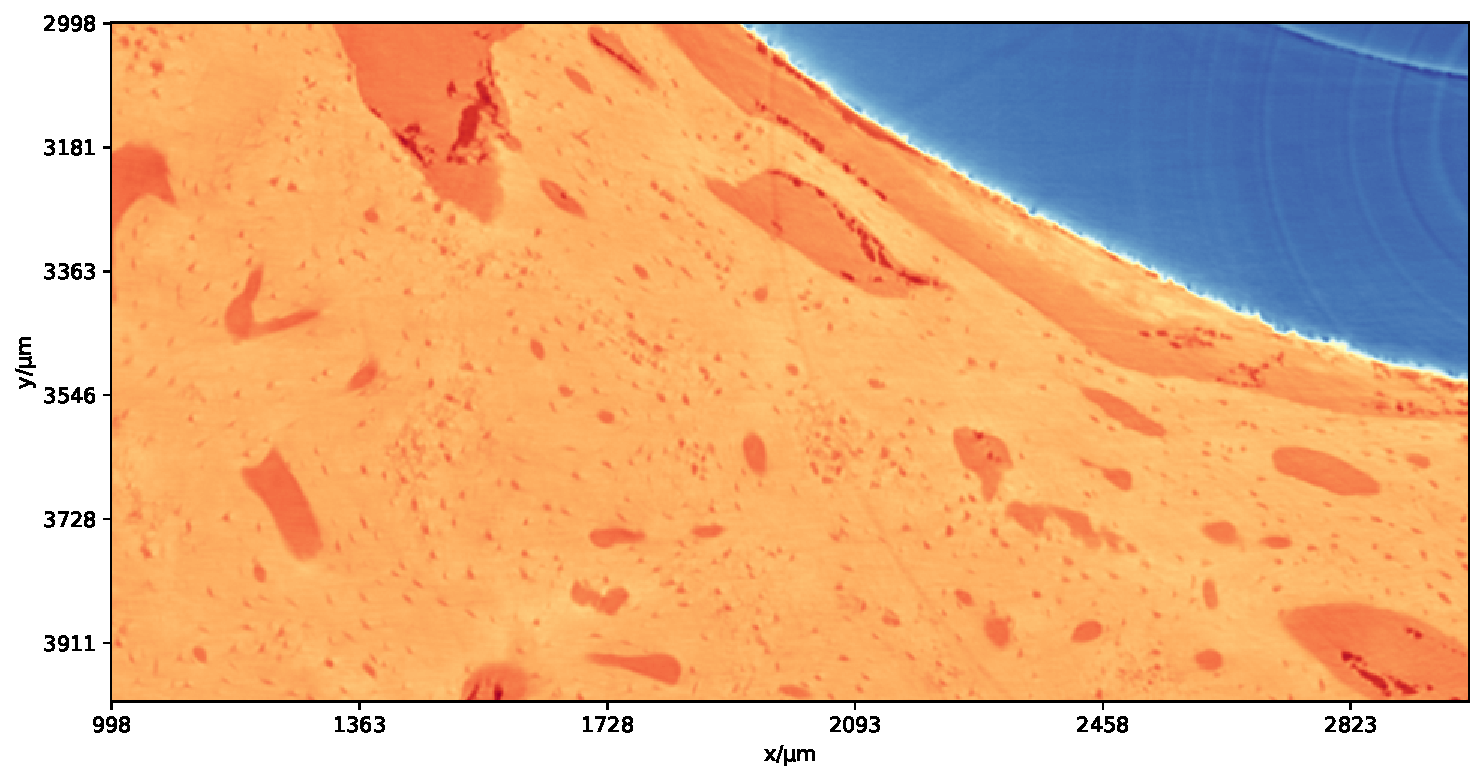
\includegraphics[width=\linewidth]{generated/770c_pag_segmented_yx_raw.pdf} \\
        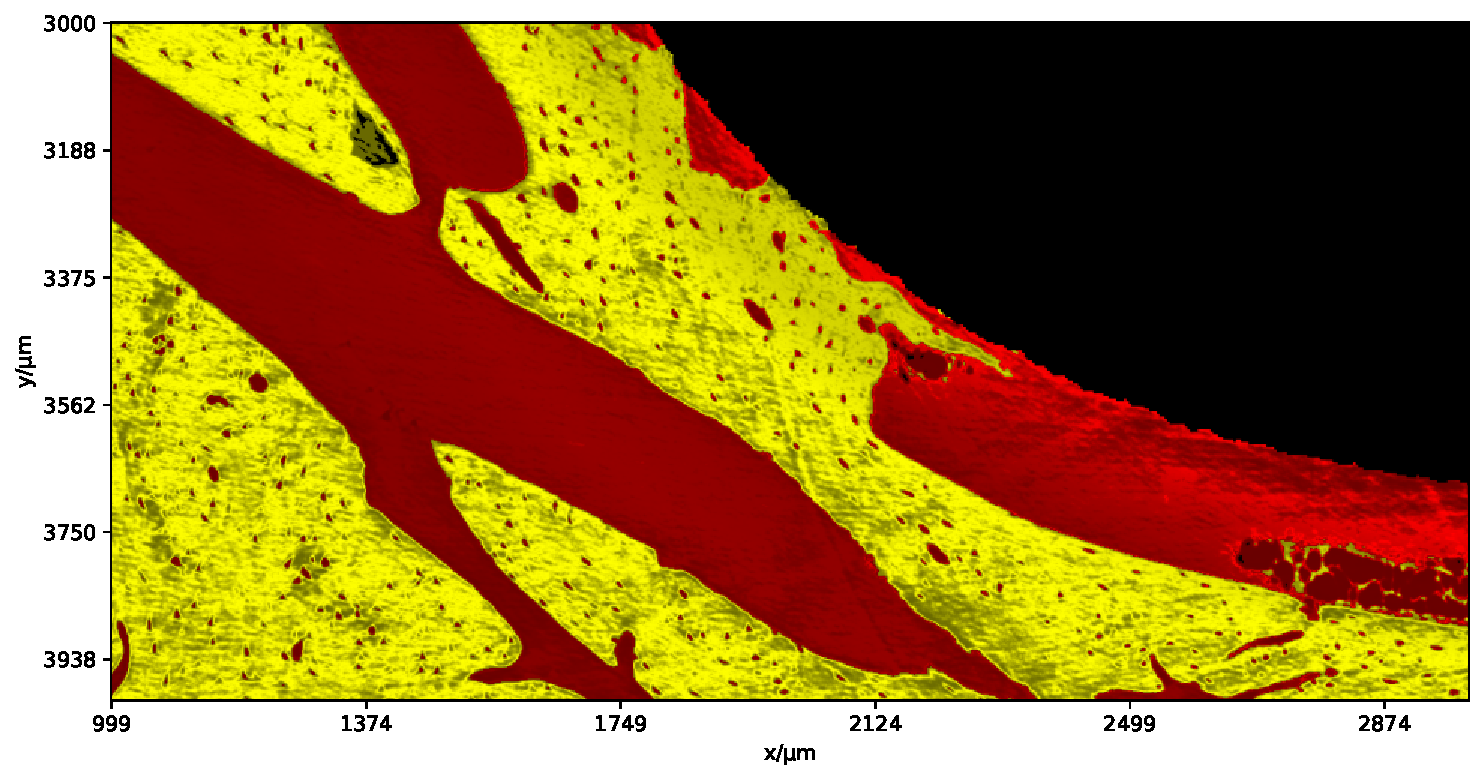
\includegraphics[width=\linewidth]{generated/770c_pag_segmented_yx_colored.pdf}
    \end{tabular}
    \caption{
        YX slices of the original tomography (top), and the classified
        (bottom). The voxels are colored according to the modeled probability
        functions $P(m\vert v,\fval)$ between 0 and 1: completely red voxels
        have $P(m=0\vert v,\fval) = 1$, completely yellow voxels have
        $P(m=1\vert v,\fval)\ = 1$, and uncertain voxels become progressively
        gray.
    }
    \label{fig:histology-comparison1}
\end{figure}

\begin{figure}
    \centering
    \begin{tabular}{c}
        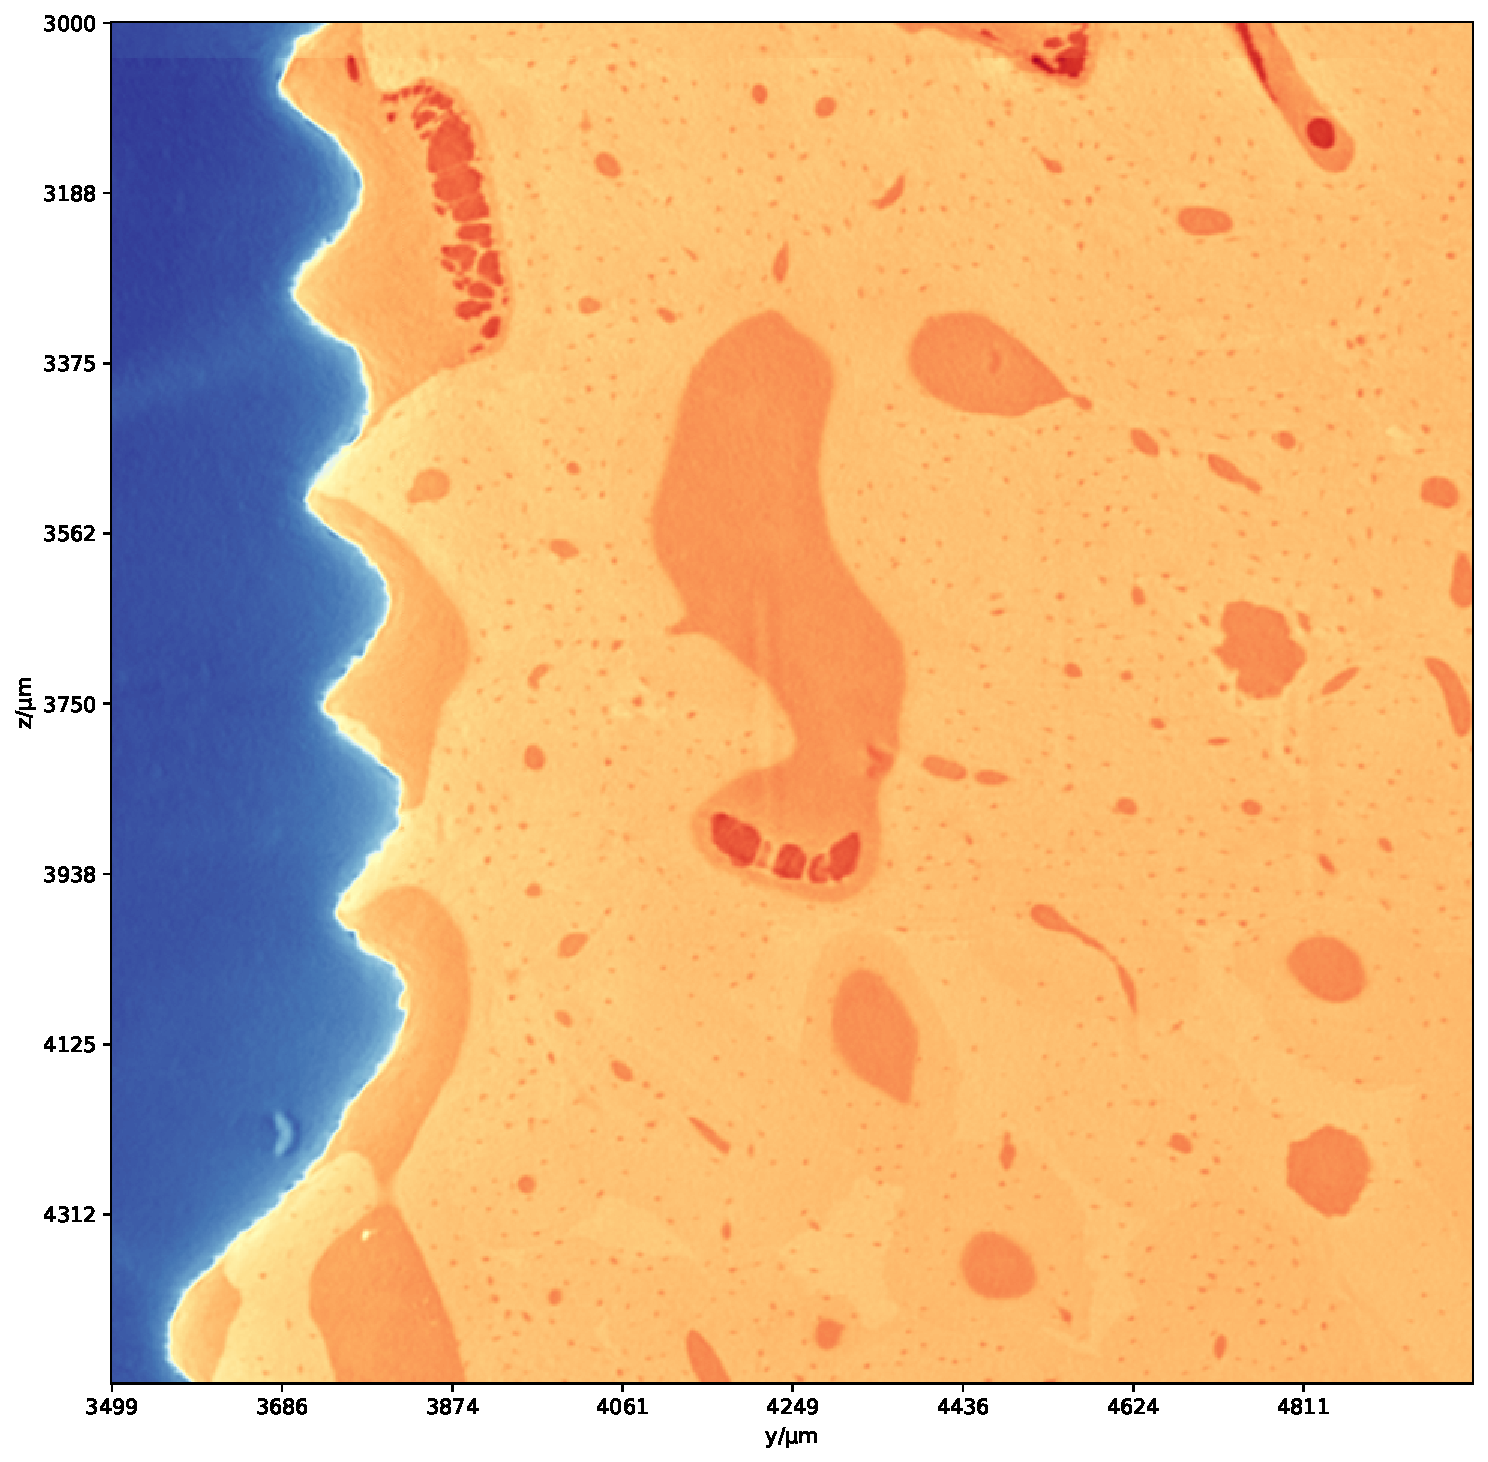
\includegraphics[width=.7\linewidth]{generated/770c_pag_segmented_zy_raw.pdf} \\
        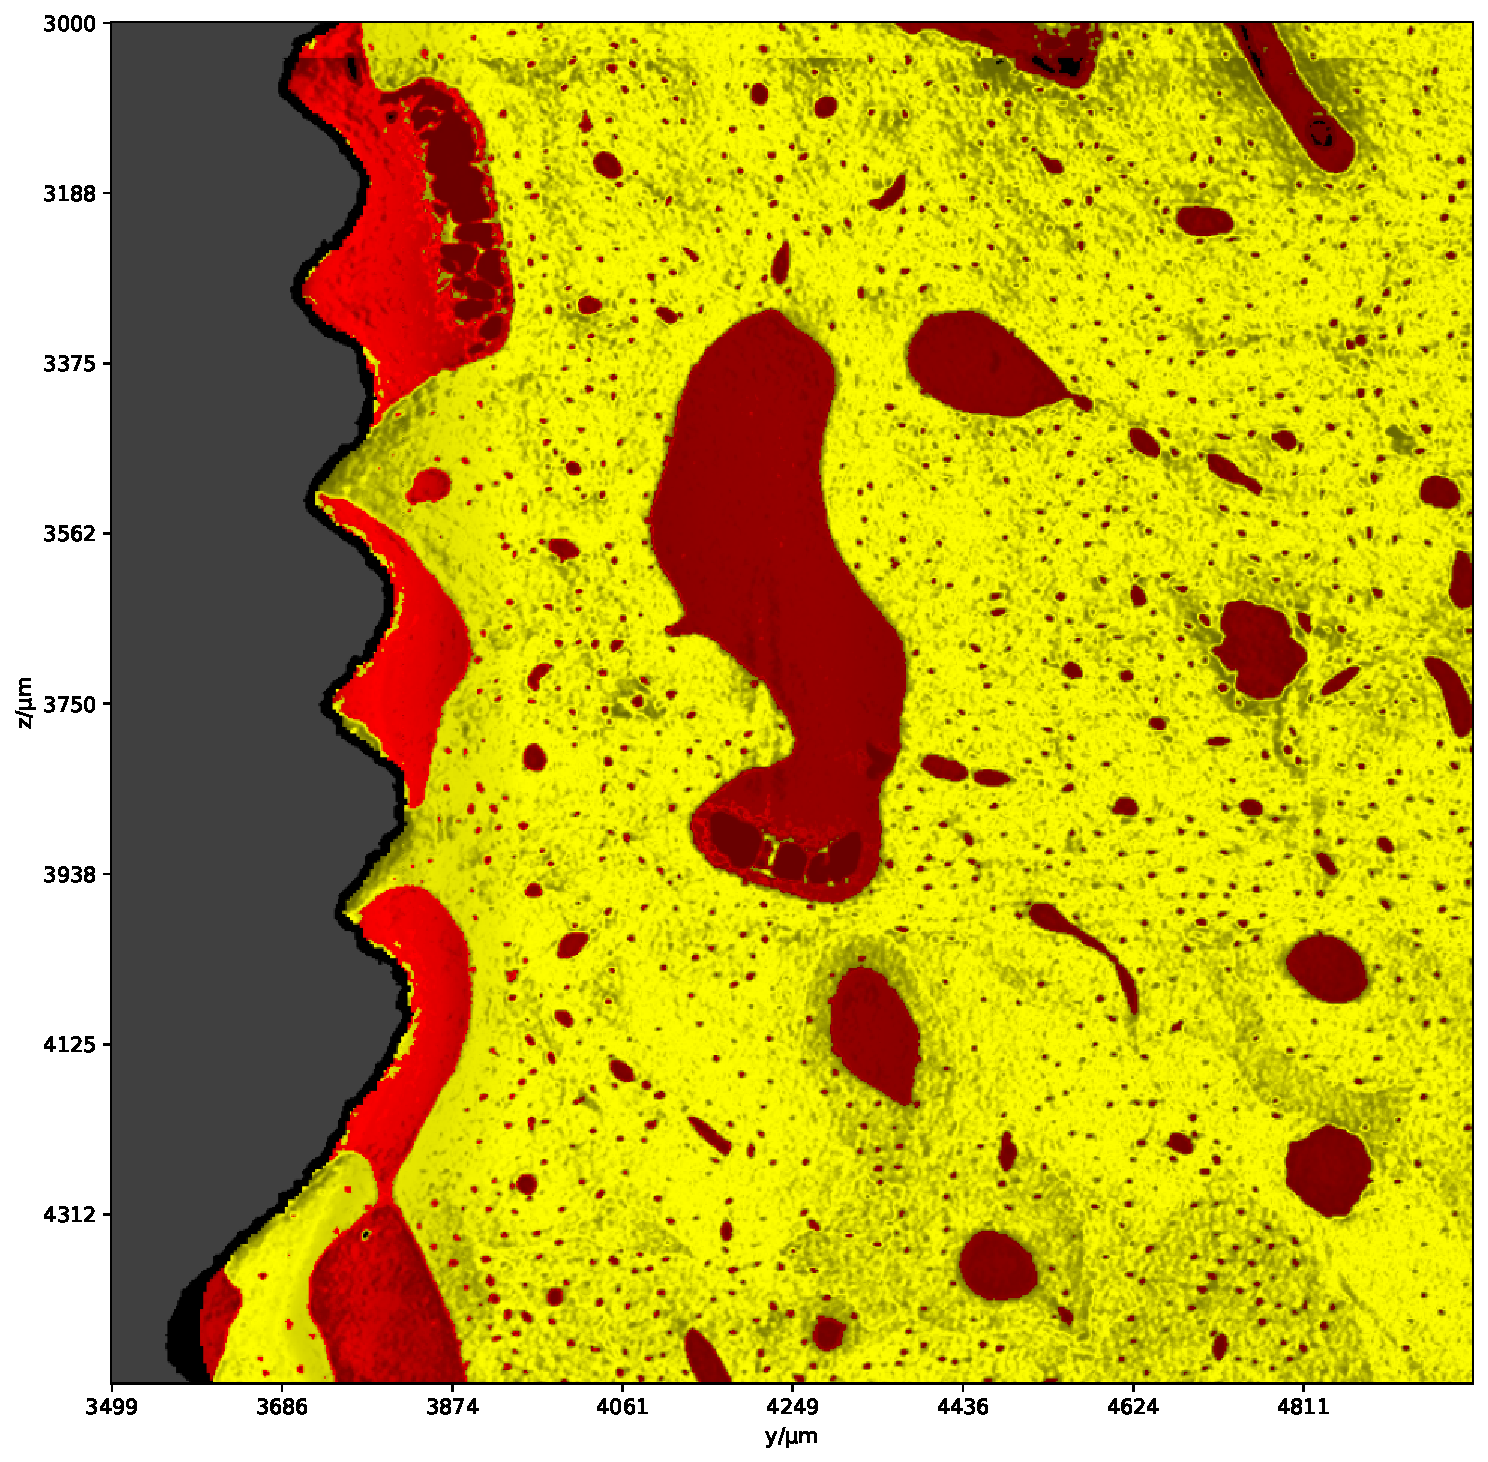
\includegraphics[width=.7\linewidth]{generated/770c_pag_segmented_zy_colored.pdf}
    \end{tabular}
    \caption{
        YZ slices of the original tomography (top) and the classified (bottom).
        Yellow depicts bone and red depicts soft tissue. Note that the
        segmentation correctly classifies the materials close to the implant,
        even in the grooves of the screw threads.
    }
    \label{fig:histology-comparison2}
\end{figure}

\subsubsection{Blood vessel network}

With a good separation of soft tissue and bone, we map out the blood vessel
network using connected components analysis, which is visualized in the 3D
renders in~\Cref{fig:blood-network}. Here we see that we have successfully
segmented the blood vessels out of the bone region. It is especially prominent
when looking at the capillary network, as we can see these in fine detail.
Noteworthy, the newly formed bone region (\Cref{fig:blood-new-slice}) contains
larger concentrations of small blood vessels, compared to the old bone
(\Cref{fig:blood-old-slice}). If we zoom in on a small cube region
(\Cref{fig:blood-old-cube} and \Cref{fig:blood-new-cube}), we see it even more
defined, clearly seeing how the larger vessels connect through the smaller
ones.

\begin{figure}
    \centering
    \begin{subfigure}[b]{\linewidth}
    \centering
        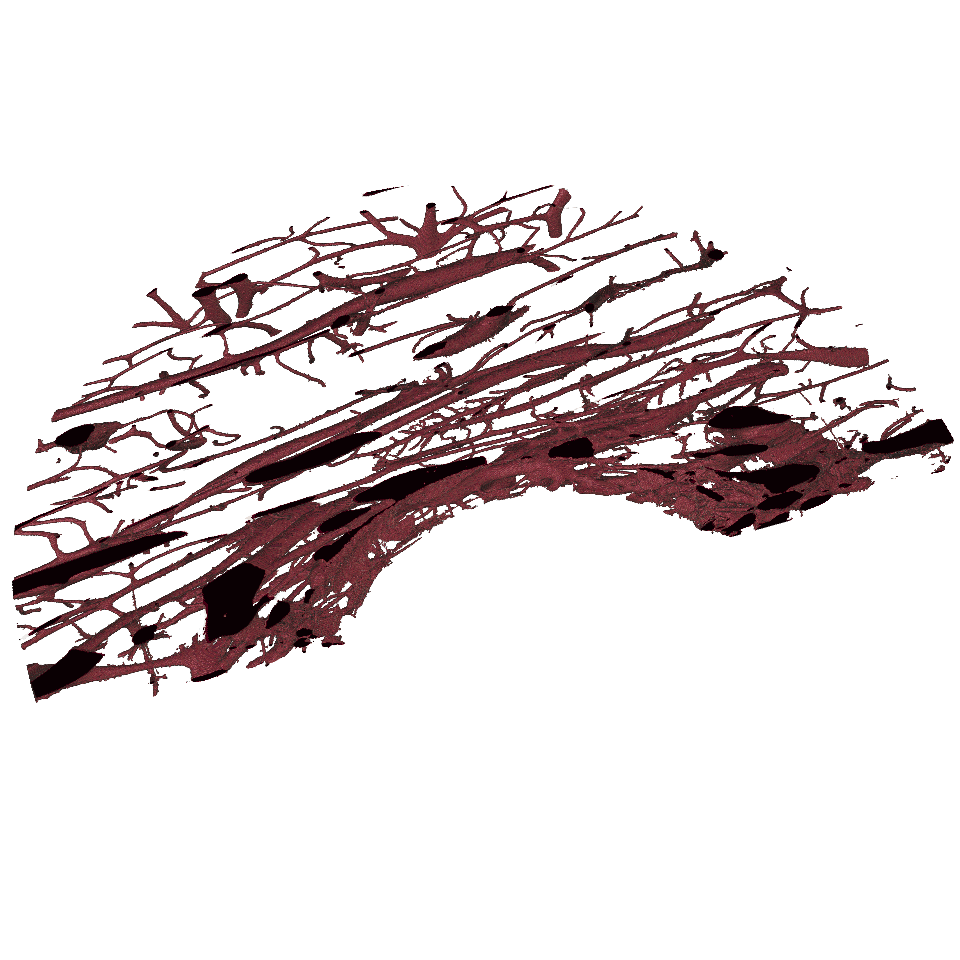
\includegraphics[width=.7\linewidth]{generated/figure10_old_bone.png}
        % TODO opdater hvis en anden slice størrelse bliver brugt. voxel size = 3.75
        \caption{A $375\mu m \times 4230\mu m \times 6480\mu m$ slice of the blood network in the old bone region.}
        \label{fig:blood-old-slice}
    \end{subfigure}
    \begin{subfigure}[b]{\linewidth}
    \centering
        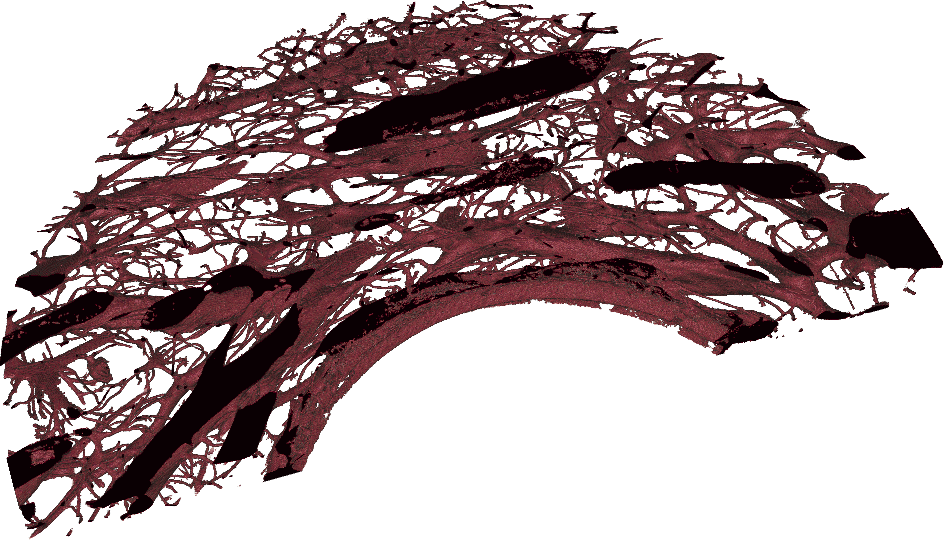
\includegraphics[width=.7\linewidth]{generated/figure10_new_bone.png}
        \caption{A $375\mu m \times 4230\mu m \times 6480\mu m$ slice of the blood network in the new bone region.}
        \label{fig:blood-new-slice}
    \end{subfigure}
    \begin{subfigure}[b]{.48\linewidth}
    \centering
        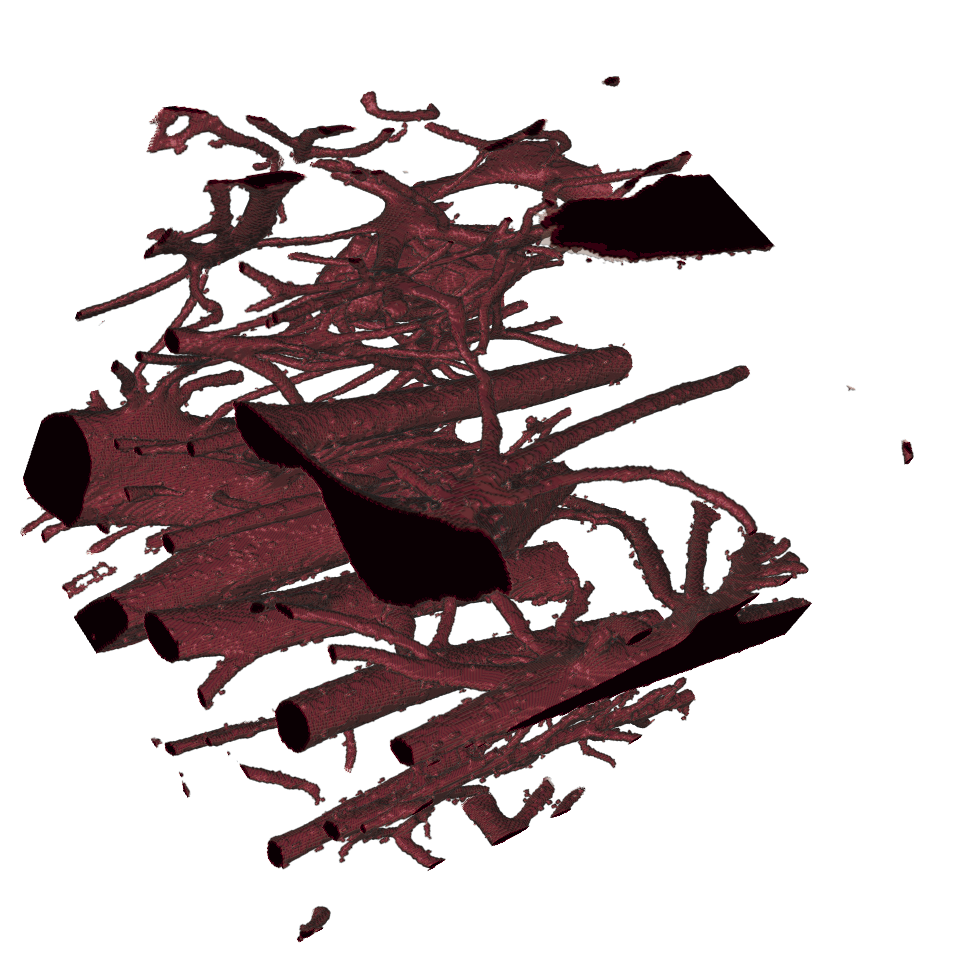
\includegraphics[width=.9\linewidth,height=\linewidth]{generated/figure10_old_cube.png}
        \caption{A $1mm \times 1 mm \times 1 mm$ cube of the blood network in the old bone region.}
        \label{fig:blood-old-cube}
    \end{subfigure}
    \hfill
    \begin{subfigure}[b]{.48\linewidth}
    \centering
        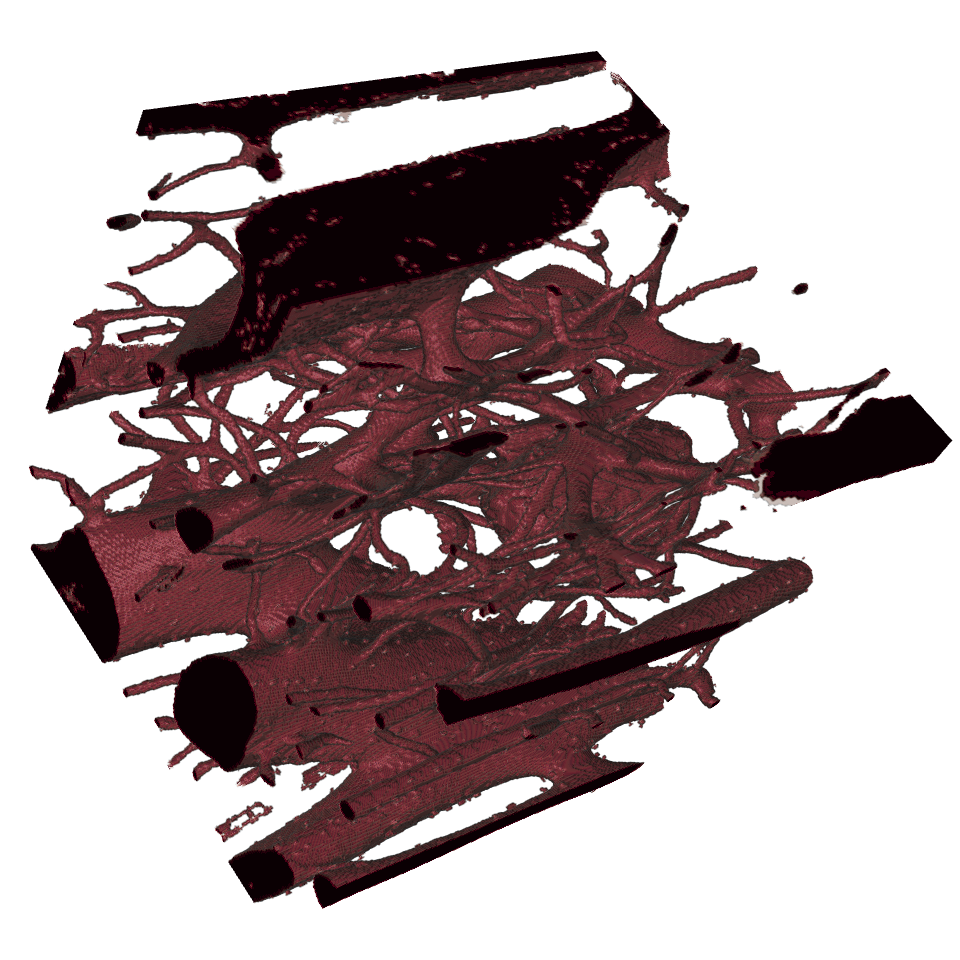
\includegraphics[width=.9\linewidth,height=\linewidth]{generated/figure10_new_cube.png}
        \caption{A $1mm \times 1 mm \times 1 mm$ cube of the blood network in the new bone region.}
        \label{fig:blood-new-cube}
    \end{subfigure}
    \caption{
        3D renders of the blood network. We see a difference between the
        capillary network in the old bone region
        (\ref{fig:blood-old-slice},\ref{fig:blood-old-cube}) compared to the
        newly grown bone region
        (\ref{fig:blood-new-slice},\ref{fig:blood-new-cube}), where the new
        bone region contains a higher concentration of small blood vessels,
        compared to the old bone region containing fewer larger blood vessels.
    }
    \label{fig:blood-network}
\end{figure}